\chapter{Analíticas automáticas en Unibotics}
\label{analiticas}
En este capítulo se explica la recogida de las sondas en Unibotics, su posterior guardado en la base de datos Elasticsearch, la visualización de dichos datos con el \textit{framework} web Dash y la validación experimental del proceso.

\section{Diseño}
Para conseguir las analíticas automáticas en Unibotics, se ha hecho un diseño de los cambios en la plataforma con las nuevas tecnologías involucradas: Elasticsearch y Dash.\\

\begin{figure}[H]
    \centering
    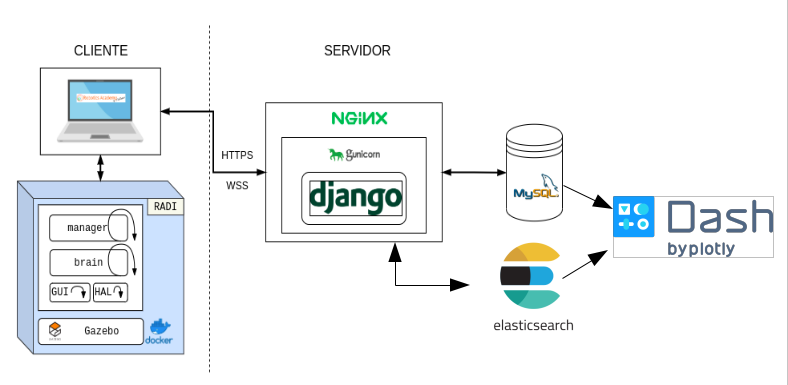
\includegraphics[width=15cm, keepaspectratio]{img/grafico.png}
    \caption{Arquitectura Unibotics con las nuevas tecnologías}
    \label{fig:grafico}
\end{figure}
En la Figura \ref{fig:grafico} se presenta la nueva arquitectura de Unibotics. Cuando un usuario interactúa con la plataforma de Unibotics, la herramienta de Elasticsearch recoge la información de éste. Las visualizaciones de las sondas recogidas se hacen a través de Dash, herramienta independiente a Django. Dash utiliza la base de datos de MySQL y Elasticsearch.\\

Lo primero que hace un usuario cuando quiere entrar en la plataforma es registrarse en ella, guardando ese registro en la base de datos MySQL. Una vez registrado, podrá iniciar sesión en ella, en el momento que desee. Cuando se encuentre dentro de la plataforma, podrá elegir un ejercicio y acceder a él, dónde podrá programar la solución. Dentro de los ejercicios tienen la opción de pedir una evaluación automática de estilo y eficacia del código programado. Para abandonar la plataforma se puede cerrar sesión o de manera implícita, cerrando el navegador o la pestaña.\\

\section{Recogida de sondas}
La primera parte de este proceso ha consistido en la recogida de diferentes sondas. Para realizar esta tarea, se ha decidido utilizar la herramienta de Elasticsearch por las ventajas que ofrece explicadas en el capítulo 3.\\

En este proyecto se ha utilizado la imagen de Docker de Elasticsearch debido a que permite que funcione en cualquier sistema operativo y replicar la instalación en cualquier máquina es directo. Primero hay que descargar la imagen de Elasticsearch con la versión deseada en este caso se ha utilizado la 7.12.0, el comando para descargar la imagen es:
{\footnotesize
		\begin{verbatim}
			docker pull docker.elastic.co/elasticsearch/elasticsearch:7.12.0
		\end{verbatim}
		}
        
Para ejecutar el contenedor con la imagen descargada se utiliza el siguiente comando:

{\footnotesize
		\begin{verbatim}
			docker run --name=AcademyElastic -p 9200:9200 -p 9300:9300
            -e "discovery.type=single-node" 
            docker.elastic.co/elasticsearch/elasticsearch:7.12.0
		\end{verbatim}
		}
\newpage
  Una vez puesto en marcha el contenedor de Elasticsearch, se tiene la base de datos donde se guardarán las sondas. Es posible realizar solicitudes directamente desde el navegador web accediendo a la URL dónde esté desplegada la base de datos, por ejemplo: \texttt{http://localhost:9200/}.\\
  
  El siguiente paso es la integración de Elasticsearch en el servidor basado en Django. Para ello se hará uso de la librería \texttt{django-elasticsearch-dsl}. Además, se ha modificado el archivo de configuración del proyecto, \texttt{settings.py}. Se ha incluido la librería a las aplicaciones instaladas y creado una nueva variable, llamada \texttt{ELASTICSEARCH\_DSL}. Se ha añadido en \texttt{settings.py}, ya que las variables declaradas en ese fichero se pueden utilizar en cualquier parte del servidor. En esa variable se indica cual es el servidor de Elasticsearch, con el que se tiene que conectar y sincronizar.\\
  
Una vez conectado Django con Elasticsearch se han definido y configurado los índices donde se guardarán las sondas. Para ello, se ha creado un nuevo archivo, llamado \texttt{probe.py}. Al definir un índice, se determinan los nombres de cada campo (información que se quiere almacenar) con el tipo de campo que es, por ejemplo: un texto, un número, una fecha, entre otros. También, se puede configurar el índice, por ejemplo, poniendo el número de\textit{ shards }o el número de réplicas. Un ejemplo de la definición de un índice sería este: 

\begin{lstlisting}
   from django_elasticsearch_dsl import Document, Date, Text, Double
   
   class SessionDocument(Document):
    		username = Text()
  	  		start_date = Date()
   			end_date = Date()
    		duration = Double()
    		client_ip = Text()
    		browser = Text()
    		country = Text()
    		alpha_2 = Text()
    		alpha_3 = Text()
    		continent = Text()
    		class Index:
        		name = 'session_log'
        		settings = {
            			'number_of_shards': 1,
           				'number_of_replicas': 0
        }
\end{lstlisting} 

Para este proyecto se han definido cuatro índices diferentes:

\begin{itemize}
\item \texttt{session\_log}: índice que recoge las sondas relativas a las sesiones. Consta de los campos de inicio y fin de sesión, duración de la sesión, la IP, el \textit{browser} (aporta información sobre el sistema operativo, navegador y dispositivo utilizado), el continente y país del usuario, así como el nombre del usuario.
\item \texttt{exercises\_log}: índice que recoge las sondas relativas a los diferentes ejercicios. Está compuesto por la fecha de entrada en un ejercicio, la fecha de salida del ejercicio, la duración total, el nombre del ejercicio y el usuario.
\item \texttt{style\_log}: índice que recoge los datos sobre la evaluación del estilo del código de los ejercicios. Este índice está formado por el campo de la fecha en la que se realiza la evaluación, el nombre del ejercicio, la puntuación sobre 100 y el nombre del usuario.
\item \texttt{efficacy\_log}: índice que recoge los datos sobre la evaluación de la eficacia del código de los ejercicios. Los campos son iguales que en el índice de \texttt{style\_log}.
\end{itemize}

Ya definidos los diferentes índices, se importan al archivo \texttt{views.py} para poder crearlos. Las sesiones de los usuarios se guardan en el índice \texttt{session\_log}. A través de las sondas creadas, podemos recoger cuando el usuario \textit{loguea} en la plataforma y cuando finaliza su actividad en ella. Se recoge la sonda de la siguiente manera:
\\
{\footnotesize
\begin{verbatim}
    probe_session = SessionDocument(username=username,start_date=datetime.now(),
                                    end_date=datetime.now(),duration=0, client_ip=ip,
                                    browser=request.META['HTTP_USER_AGENT'],
                                    country=location_info["country_name"],
                                    alpha_2=location_info["alpha_2"], 
                                    alpha_3=location_info["alpha_3"],
                                    continent=location_info["continent"])
    probe_session.save()
\end{verbatim}
}
\newpage
Gracias al objeto HTTP Request que recibe el fichero \texttt{views.py}, se obtiene la información del nombre del usuario, la IP y el \textit{user-agent}. En el \textit{user-agent} se encuentra el sistema operativo, el navegador o el dispositivo que utiliza el usuario. Para la localización se ha creado una función que, a partir de la IP, muestra la ubicación. Cuando el usuario \textit{loguea}, los campos de fin de sesión y duración se inicializan con la fecha actual y 0 respectivamente, una vez que el usuario haga \textit{logout} o finalice su sesión por inactividad estos campos se modificarán como se muestra a continuación:\\
{\footnotesize
\begin{verbatim}
    s = Search(index="session_log").query('match', username=request.user.username) \
                                    .sort({"start_date": {'order':'desc'}})[0]
    for hit in s:
        end = datetime.now()
        Elasticsearch(settings.ELASTICSEARCH_DSL['default']['hosts']) \
                        .update(index="session_log", id=hit.meta.id,
                                body={"doc": {'end_date': end,
                                'duration':(end - datetime \
                                    .strptime(hit.start_date,'%Y%m%dT%H:%M:%S.%f')) \
                                    .total_seconds()}})
\end{verbatim}
}
\\
Las sondas relativas a los ejercicios se guardan cuando el usuario accede a un ejercicio. Como ocurre con las sesiones, cuando el usuario abandone el ejercicio se modificarán los datos de duración y fin del ejercicio. Se ha tenido en cuenta que al recargar un ejercicio en el que el usuario ya se encontraba, no se cree una sonda nueva y se tenga en cuenta la primera sonda creada para dicho ejercicio. Las sondas no deseadas que se han creado se eliminan de la siguiente forma:\\
\\
{\footnotesize
\begin{verbatim}
   es = Search(index="exercises_log").query('match', duration=0)  \
   				            .query('match', username=request.user.username)  \
        					                .sort({"start_date": {'order':'desc'}})
    for hit in es:
        Elasticsearch(settings.ELASTICSEARCH_DSL['default']['hosts'])  \ 
    				                        .delete(index="exercises_log", id=hit.meta.id)
\end{verbatim}
}
\newpage
Cada ejercicio que se encuentra en Unibotics dispone de un botón de evaluación automática de estilo, donde se dan unas recomendaciones para mejorar el estilo del código del usuario y una puntuación. La puntuación es recogida en el índice de \texttt{style\_log}. Para poder recoger la puntuación recibida en la evaluación de eficacia, se ha creado un nuevo botón en los ejercicios. Una vez pulsado el botón, empieza a ejecutar el código durante un tiempo determinado, según el ejercicio. Pasado ese tiempo se obtiene la nota obtenida del ejercicio y se guarda en el índice de \texttt{efficacy\_log}. Si el usuario pulsa dos veces al botón, se considera que el usuario no desea la evaluación automática, por lo cual la sonda no se guardará.\\


En este proceso de recogida de sondas y su grabación ha sido muy útil la utilización de la API que proporciona Elasticsearch para poder depurar y comprobar los datos que se estaban almacenando. Utilizando por ejemplo la URL    \newline       \texttt{http://127.0.0.1:9200/session\_log/\_search/?size=10000&pretty}, se comprueba las sondas de sesiones.\\

Las sondas recogidas han estado en producción desde el 5 de mayo de 2021. Como resultado, se ha obtenido la información de usuarios reales desde esa fecha.\\

Para comprobar el funcionamiento de Elasticsearch se generaron datos de prueba para poder comenzar a trabajar antes de tener los datos reales, los cuales llevan tiempo recoger. La base de datos Elasticsearch dummy se ha creado gracias a las librerías de Python Faker\footnote{https://faker.readthedocs.io/en/master/} y Tornado\footnote{https://www.tornadoweb.org/en/stable/} en ella se puede modificar las sondas. Por ejemplo, el número de sondas, de réplicas o de \textit{shards}. Esto ayudará a futuros desarrolladores a utilizar la base de datos de Elasticsearch. En la Figura\ref{fig:dummy} se muestra el resultado de la sonda de evaluación de estilo de la base de datos de prueba.


\begin{figure}[H]
    \centering
    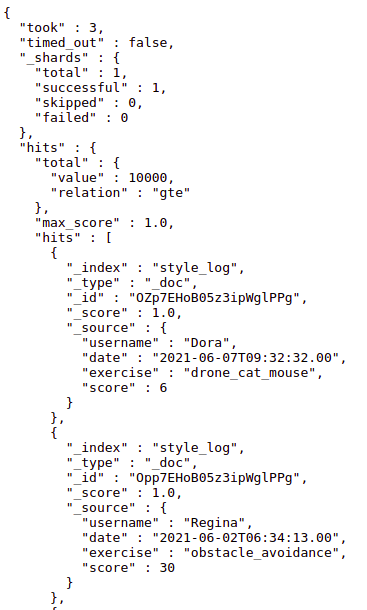
\includegraphics[width=6cm, keepaspectratio]{img/dummy.png}
    \caption{Elasticsearch dummy}
    \label{fig:dummy}
\end{figure}

\section{Visualización de la información}

Dash es un \textit{framework} web que permite crear tableros web interactivos con visualizaciones dinámicas, para poder hacer análisis como se explica en el capítulo 3. En este Trabajo de fin de grado se ha decidido utilizar esta herramienta para la visualización de las sondas recogidas en Elasticsearch.\\

Solo los usuarios registrados en Unibotics podrán acceder a las visualizaciones. Dependiendo del tipo de usuario, se tiene disponible unas visualizaciones u otras. Para iniciar sesión, se ha hecho uso de los usuarios ya guardados en la base de datos MySQL de la que depende Django, en la que se encuentra la información sobre el tipo de usuario (\textit{staff}, \textit{admin}, \textit{user}...). En el caso de los administradores podrán ver la información de todas las sondas, mientras que un usuario de Unibotics solo podrá acceder a las puntuaciones de estilo y de eficacia obtenidas en cada ejercicio. En la Figura \ref{fig:menu} muestra el menú disponible para los administradores.

\begin{figure}[H]
    \centering
    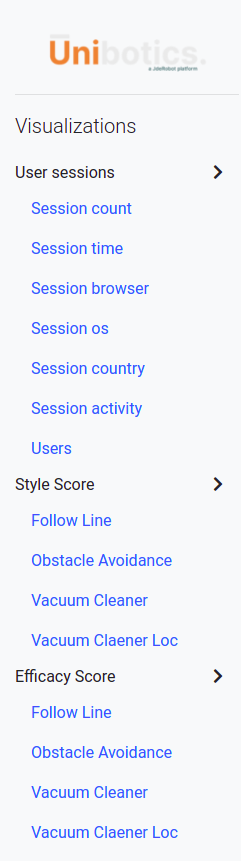
\includegraphics[width=3cm, keepaspectratio]{img/menu.png}
    \caption{Menú de un administrador en Dash}
    \label{fig:menu}
\end{figure}


Gracias a las bibliotecas de Dash, mencionadas en el capítulo 3, se ha dado estilo y formato a la aplicación. También, se ha hecho uso de las \textit{cookies }del navegador, guardadas al inicio de sesión de Dash, para comprobar si se está autorizado y si es un administrador de la plataforma.\\

Dash trabaja con dataframes, por lo que es necesario realizar una primera transformación de los datos de Elasticsearch a esta estructura, gracias a la biblioteca de Pandas. Un ejemplo de la realización de esta conversión es:

{\footnotesize
\begin{verbatim}
  s = Search(using=es, index="session_log")
  results = [hit.to_dict() for hit in s.scan()]
  df  = pd.DataFrame(results)
\end{verbatim}
}
\\
\\
Con la biblioteca \texttt{dash\_core\_components} se han creado los filtros que algunas de las gráficas poseen. Estos filtros de forma dinámica, cambian las visualizaciones en base a dicho filtrado. Uno de los filtros que más se ha utilizado es el filtro por fechas. Estableciendo una fecha de inicio o de fin o ambas. Es posible conocer la situación de Unibotics en un periodo de tiempo concreto. El código de filtrado es:

{\footnotesize
\begin{verbatim}
 if start_date is not None and end_date is not None:
        df=df.loc[(df['start_date'] > start_date) & (df['start_date'] <= end_date)]
elif start_date is not None:
        df=df.loc[(df['start_date'] > start_date)]
elif end_date is not None:
        df=df.loc[(df['start_date'] <= end_date)]
\end{verbatim}
}
\\

Otro filtro recurrente en la mayoría de las visualizaciones es el filtro por usuario. Este filtro solo aparece en las gráficas accesibles por los administradores, de forma que se puedan visualizar los datos de los diferentes usuarios de la plataforma. Para este filtro se hace uso de las sondas de sesiones, recogiendo los nombres de los usuarios de forma única y añadiendo un 'Total' en los casos que se quiera visualizar las sondas de todos los usuarios. En resumen, el filtro podrá filtrar por usuario único, un grupo de usuarios o por el total de los usuarios, \newline\texttt{df = df[df.username.isin(user)]} . El código para conseguir los nombres de los usuarios y añadir la opción de 'Total', es el siguiente:

{\footnotesize
\begin{verbatim}
	s = Search(using=es, index="session_log")
    results = [hit.to_dict() for hit in s.scan()]
    df  = pd.DataFrame(results)
    df = df[df['username'].notna()]
    users = df['username'].unique()
    if not exercises:
        users = np.insert(users,0,'Total')
    return users
\end{verbatim}
}
\\
\begin{figure}[H]
    \centering
    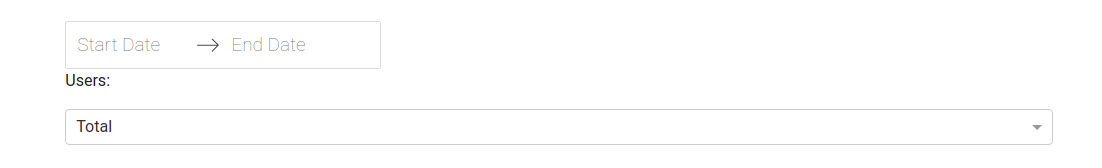
\includegraphics[width=16cm, keepaspectratio]{img/filtros.png}
    \caption{Filtros utilizados en Dash}
    \label{fig:filtros}
\end{figure}

Dash utiliza el módulo Plotly para generar las visualizaciones. Plotly ofrece una gran variedad de gráficas que se pueden utilizar en Dash. Adicionalmente se puede combinar varias gráficas en los mismos ejes, haciendo más sencilla la correlación entre datos.\\

\\
En las siguientes subsecciones, se detallan los resultados finales de las analíticas con datos reales de la plataforma de Unibotics. Se muestran las diferentes gráficas creadas tanto para administradores como para los usuarios, así como una explicación de lo que representan.
\subsection{Registros y usuarios de la plataforma}
Los administradores tienen la opción de poder ver el número total de usuarios que son activos, el número de usuarios que han sido activos en los últimos 2 meses, en formato numérico. Además, se muestra las gráficas de línea de registros por cada día, registros acumulados por días (Figura \ref{fig:accumulated}) y usuarios activos en los últimos 2 meses (Figura \ref{fig:active}). Cada una de estas gráficas contiene su propio filtrado por fechas.\\

Para la gráfica de usuarios activos, empezando por la primera sesión recogida en
\texttt{session\_log} hasta el día actual, se comprueba cuantos usuarios han iniciado sesión desde 2 meses atrás hasta el día que se está comprobando. El código para crear una gráfica de línea es el siguiente, en este caso del número de usuarios activos por día:
\begin{verbatim}
def get_temporal_figure_active_users(df):
    fig = px.line(df, x='Date', y='Active Users')
    fig.add_trace(go.Scatter(x=df["Date"].tolist(), 
                             y=df["Active Users"].tolist(),
                             mode="markers", textposition="top center", 
                             name="Active Users",
                             text=df["Active Users"].tolist()))
return fig
\end{verbatim}
\\
Las gráficas de las Figuras \ref{fig:users} y \ref{fig:accumulated} han sido elaboradas con la base de datos MySQL. Se ha realizado una lista de todas las fechas de los registros en Unibotics. Esta lista se ha convertido en dataframes. Se ha contado el número de repeticiones de cada fecha y su acumulación, dando como resultado dichas gráficas.\\



\begin{figure}[H]
    \centering
    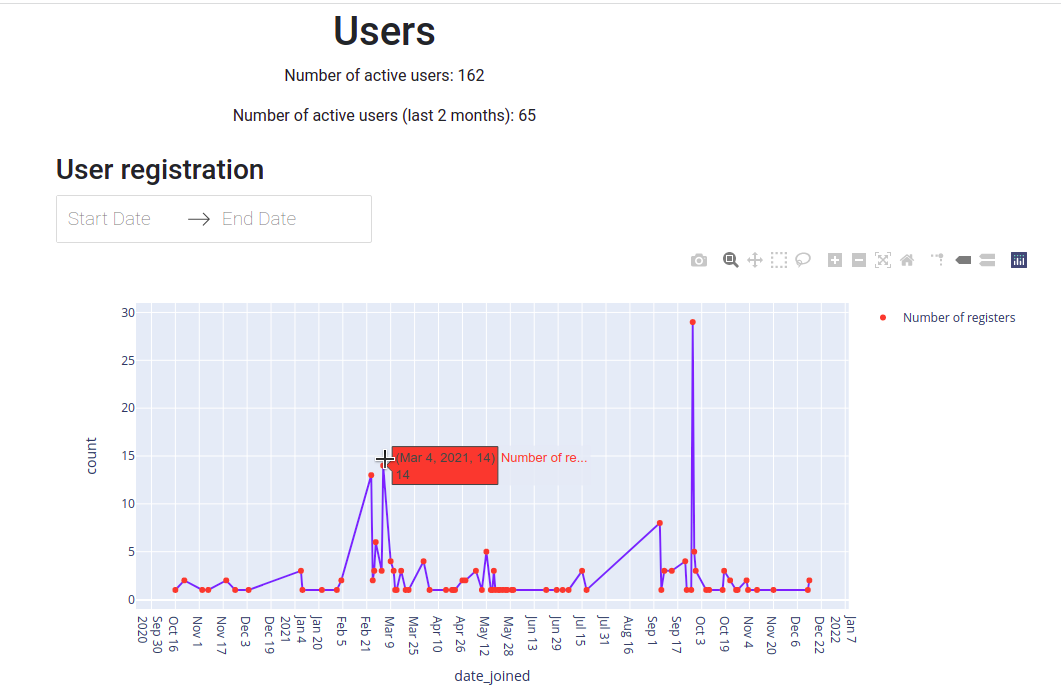
\includegraphics[width=16cm, keepaspectratio]{img/users.png}
    \caption{Gráficas relativas a los usuarios}
    \label{fig:users}
\end{figure}
\begin{figure}[H]
    \centering
    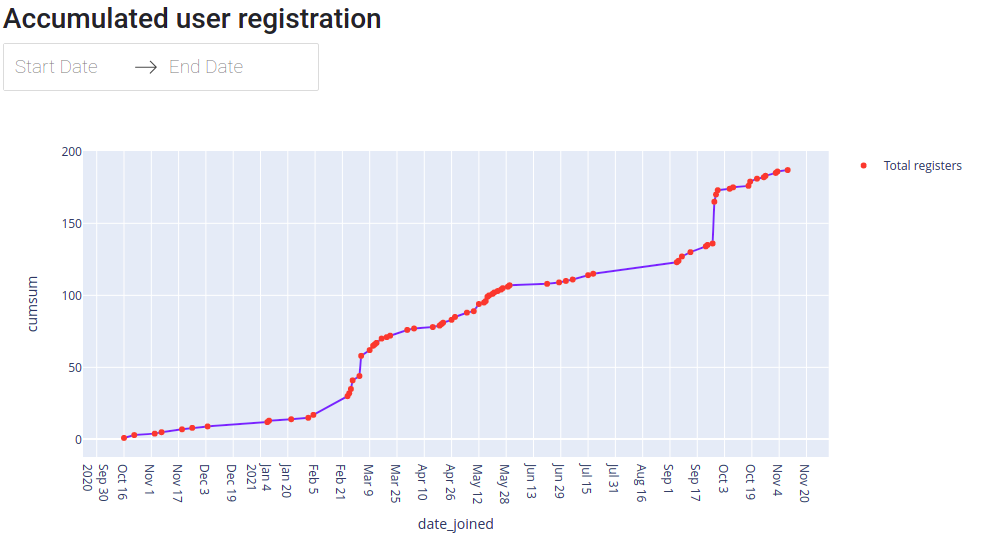
\includegraphics[width=16cm, keepaspectratio]{img/accumulated.png}
    \caption{Gráfica registro de usuarios acumulado}
    \label{fig:accumulated}
\end{figure}
\begin{figure}[H]
    \centering
    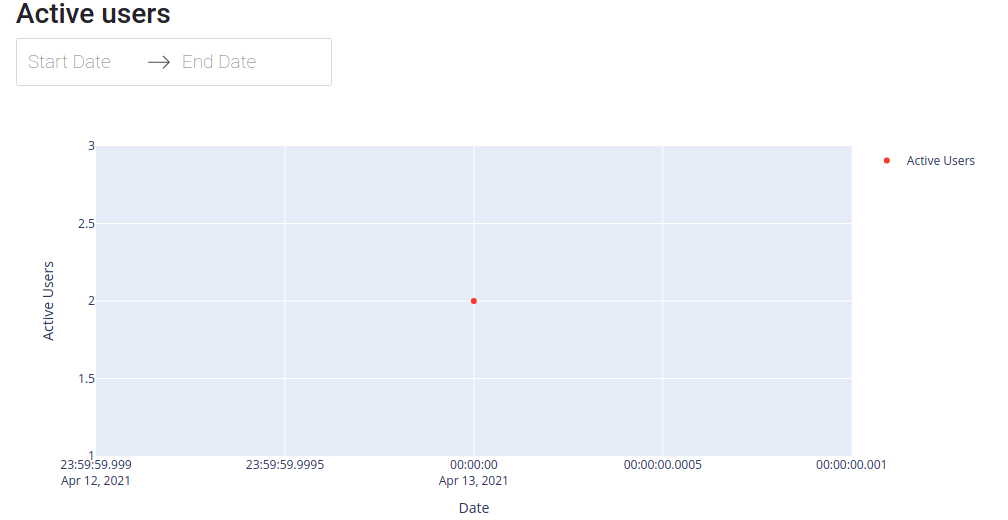
\includegraphics[width=16cm, keepaspectratio]{img/active.png}
    \caption{Gráfica de usuarios activos cada día}
    \label{fig:active}
\end{figure}

En todas las gráficas de Dash si se pone el cursor sobre uno de los puntos se puede ver la información con mayor detalle, como se muestra en la Figura \ref{fig:users}. Además, Dash añade varias opciones para interactuar con la gráfica, por ejemplo, se puede descargar la gráfica, hacer \textit{zoom} o seleccionar una parte de ella. \\
\subsection{Actividad en la plataforma}

La gráfica creada que se muestra en la Figura \ref{fig:sesion}, representa en el eje x el tiempo y en el eje y el número de sesiones, dando como resultado una gráfica de linea, con énfasis en los puntos para una mejor visualización. Esta gráfica muestra el número de sesiones por día. En la gráfica se observa que días ha habido más \textit{logins}, viéndose como en los meses de verano dicho número se ha reducido. Hace uso del índice \texttt{session\_log}, contando cuantas veces el campo \texttt{start\_date} se repite.\\



\begin{figure}[H]
    \centering
    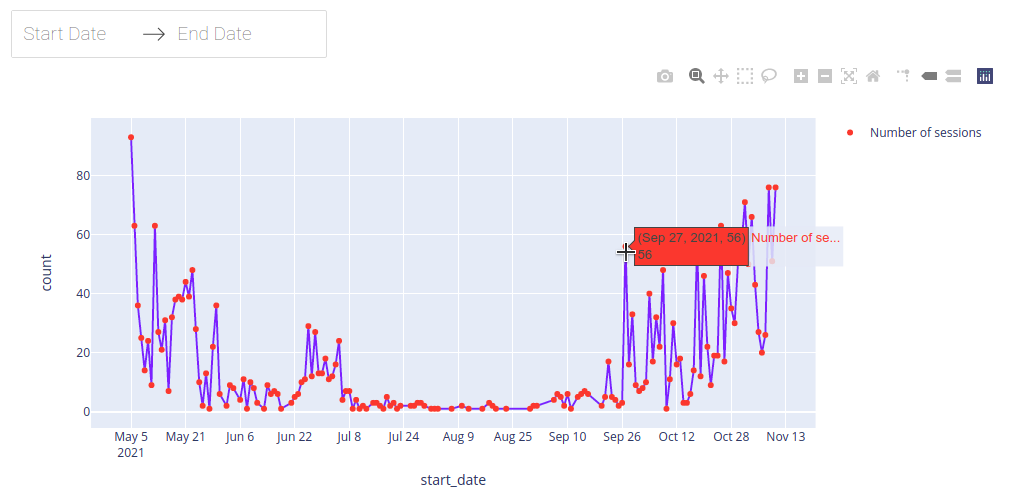
\includegraphics[width=16cm, keepaspectratio]{img/sesion.png}
    \caption{Gráfico sesiones totales por día}
    \label{fig:sesion}
\end{figure}
Se ha creado otra gráfica lineal de sesiones por día, pero en este caso solo se tiene en cuenta el número de sesiones por usuario único. La gráfica está creada de la misma manera que la gráfica del total de sesiones por día y con los mismos filtros (fechas y usuarios). Para que sean usuarios únicos, se ha eliminado los dataframes cuya columna de \texttt{username} se repetía. En la Figura \ref{fig:sesion_users}  se muestra una parte ampliada de dicha gráfica.\\

\begin{figure}[H]
    \centering
    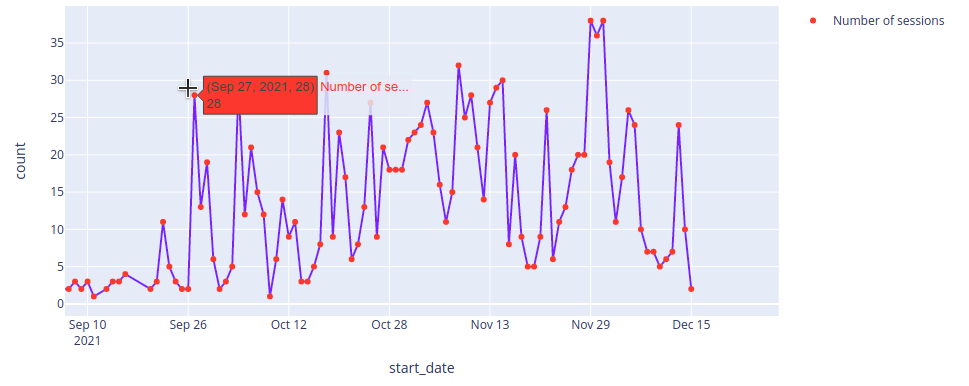
\includegraphics[width=16cm, keepaspectratio]{img/sesion_users.png}
    \caption{Gráfico sesiones únicas por día}
    \label{fig:sesion_users}
\end{figure}
La Figura \ref{fig:time} muestra una gráfica de barras en la cual se representa el tiempo mediante el eje x y la duración total de la sesión de los usuarios en minutos en el eje y. Además, se ha incluido una media que representa la duración media de las sesiones. Aquí podemos comprobar que a veces la media coincide con la duración total debido a que solo ha tenido que haber una sesión en ese día. Para realizar esta gráfica se ha utilizado los campos de \textit{duration} y \texttt{start\_date} del índice \texttt{session\_log}. Para crear la gráfica de barras junto con la gráfica de linea de la media, se utiliza el siguiente código:

\begin{verbatim}
def get_temporal_figure__session_time(df):
    fig = px.bar(df, x='start_date', y='duration')
    fig.add_trace(go.Scatter(x=df['start_date'], 
                              y=df['mean'], 
                              line=dict(color='red'), 
                              name='Mean'),
                  row=1, col=1)
    return fig
\end{verbatim}

\begin{figure}[H]
    \centering
    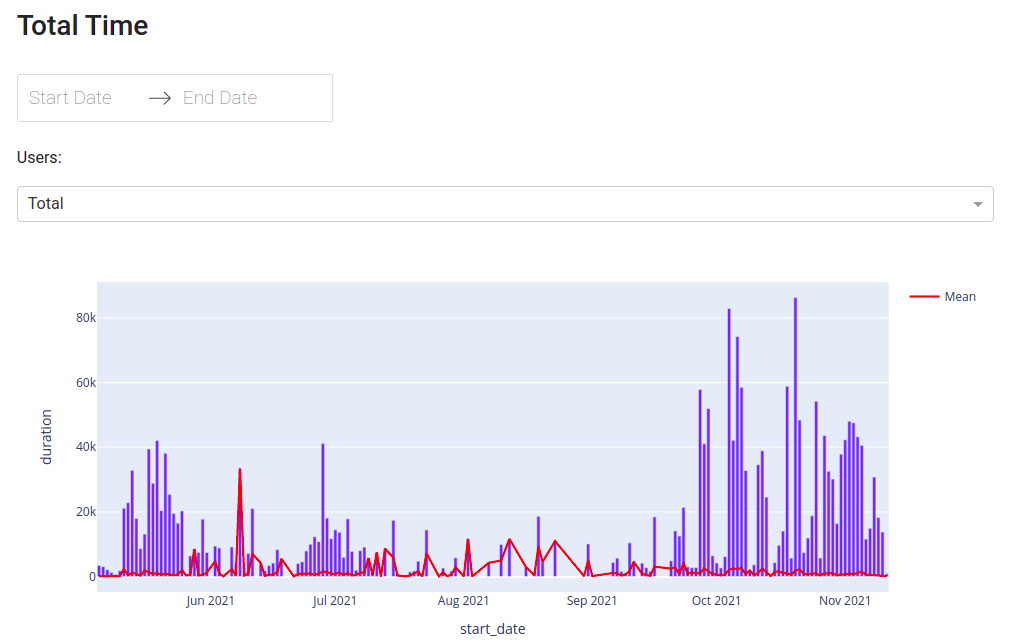
\includegraphics[width=16cm, keepaspectratio]{img/time.png}
    \caption{Gráfico de tiempo en Unibotics}
    \label{fig:time}
\end{figure}
Esta gráfica se puede filtrar tanto por fechas como por usuarios, pudiendo ver el tiempo dedicado de un usuario y la media total del tiempo que usa Unibotics dicho usuario, como se puede ver en la Figura \ref{fig:time_user}.

\begin{figure}[H]
    \centering
    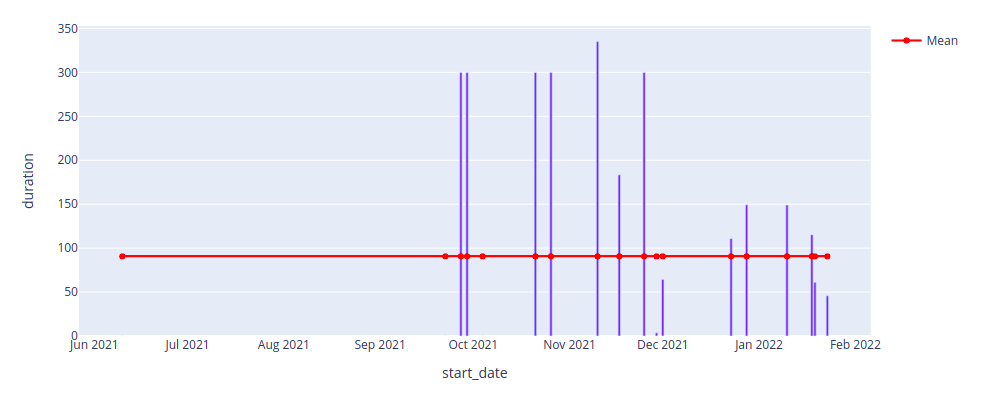
\includegraphics[width=14cm, keepaspectratio]{img/time_user.png}
    \caption{Gráfico de tiempo en Unibotics de un usuario}
    \label{fig:time_user}
\end{figure}

A fin de poder hacer un análisis de la media, la desviación típica o la moda se ha creado un histograma de las duraciones de las sesiones como se ve en la Figura \ref{fig:time_user}. En el eje x, se encuentran los diferentes intervalos de duraciones de los usuarios. En el eje y, representa cuantos usuarios han utilizado la plataforma durante el mismo tiempo. Para hacer el histograma de duración, se ha utilizado el código:
\begin{verbatim}
def get_temporal_figure__histogram_time(df):
    fig = px.histogram(df, x='duration')
    fig.update_layout(bargap=0.1)
return fig
\end{verbatim}

\begin{figure}[H]
    \centering
    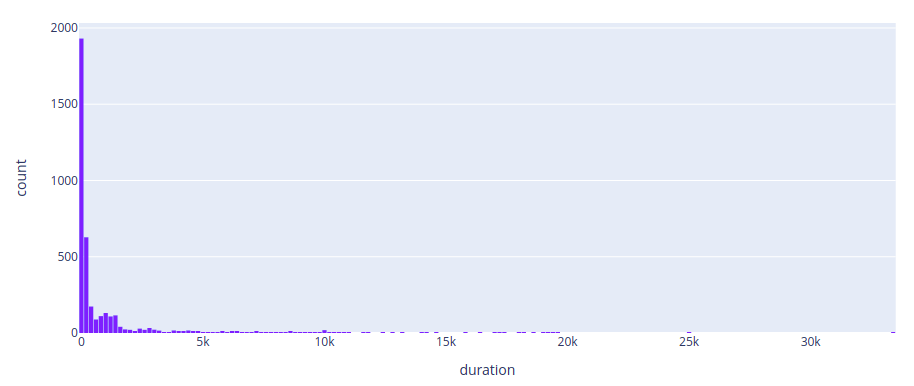
\includegraphics[width=15cm, keepaspectratio]{img/time_histogram.png}
    \caption{Histograma de las duraciones de sesiones}
    \label{fig:time_histogram}
\end{figure}
\newpage
En la siguiente gráfica que se ve en la Figura \ref{fig:activity} representa un mapa de calor con la actividad de los usuarios. Está dividido en cuadrados que representan cada día de un año, cuanto más intenso es el color verde más sesiones ha habido. Ha medida que disminuyen las sesiones la intensidad también baja. A parte del filtrado por fechas, tiene un filtro por usuario para ver la actividad por usuarios únicos o grupo de ellos. Como ocurría con la gráfica lineal de sesiones, el primer mapa de color cuenta el total de las sesiones y el segundo mapa de color cuenta las sesiones únicas por usuario. Las sesiones se han contado a través del campo de \textit{start\_date} del índice de \texttt{session\_log}.


\begin{figure}[H]
    \centering
    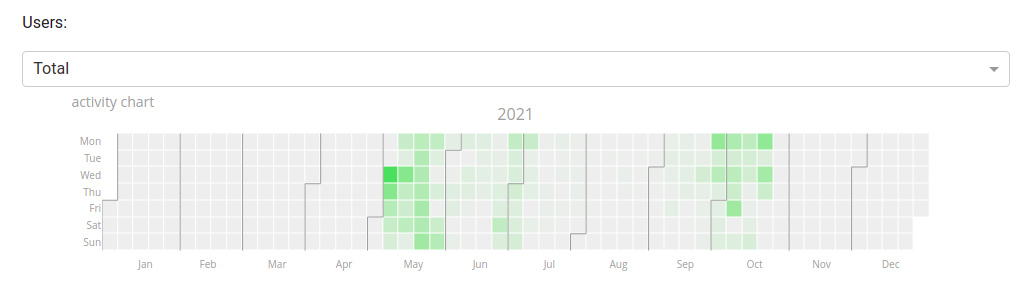
\includegraphics[width=17cm, keepaspectratio]{img/activity.png}
    \caption{Mapas de calor sesiones}
    \label{fig:activity}
\end{figure}
\newpage
En la Figura \ref{fig:mundo} se muestra un mapa geográfico con la localización de los usuarios que acceden a Unibotics. El tamaño de los puntos depende de la cantidad de sesiones, cuanto mayor sea el punto más sesiones hay. A la derecha se encuentra una leyenda con los países, se puede seleccionar uno o varios países en la leyenda para que solo se vean ellos en el mapa. Se puede filtrar por fechas. Para esta gráfica, se ha necesitado los campos de \textit{country}, \textit{continent} y \textit{alpha\_3} (código de los países), del índice de \texttt{session\_log}. Para hacer el mapa se necesita el siguiente código:
\begin{verbatim}
def get_temporal_figure__country(df):
    fig = px.scatter_geo(df, locations="alpha_3", color="country",
                     hover_name="country", size="count",
                     projection="natural earth")
return fig
\end{verbatim}


\begin{figure}[H]
    \centering
    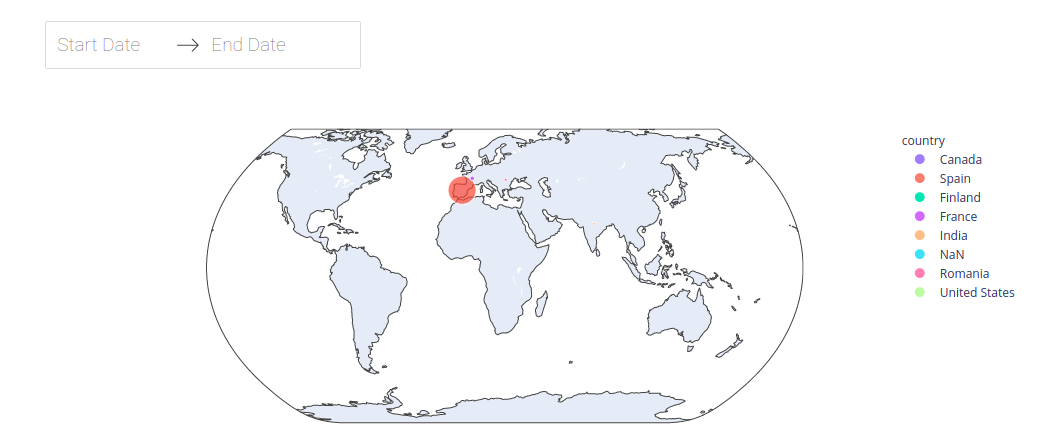
\includegraphics[width=17cm, keepaspectratio]{img/mundo.png}
    \caption{Mapa geográfico de sesiones}
    \label{fig:mundo}
\end{figure}
\newpage
Con el propósito de conocer el tiempo que invierten los usuarios en cada ejercicio se ha elaborado un histograma de las duraciones de los ejercicios. Esta gráfica dispone de un filtro del ejercicio que se desea comprobar, con el filtro de usuario y el de fechas. Por ejemplo, la Figura \ref{fig:histogram_exercise} es un histograma del ejercicio \textit{follow\_line}  de un grupo de usuarios y unas fechas concretas. Para realizar el histograma, se ha utilizado el índice de \texttt{exercises\_log}, en concreto los campos de \textit{exercise} y \textit{duration}.

\begin{figure}[H]
    \centering
    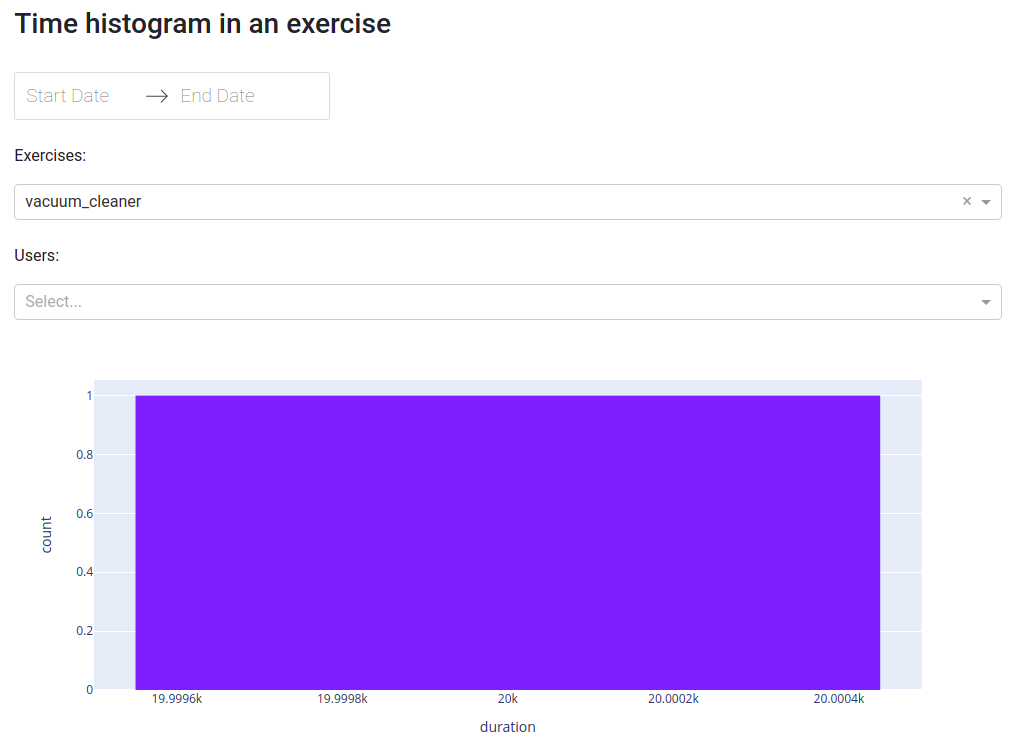
\includegraphics[width=17cm, keepaspectratio]{img/histogram_exercise.png}
    \caption{Histograma del ejercicio follow\_line de un grupo de usuarios }
    \label{fig:histogram_exercise}
\end{figure}
\newpage
\subsection{Acceso de los usuarios}
La Figura \ref{fig:browser} muestra una gráfica con los distintos navegadores que utilizan los usuarios para acceder a Unibotics, en formato porcentaje. En este caso se ve que una gran parte de inicio de sesiones es a través del navegador de Chrome. 


\begin{figure}[H]
    \centering
    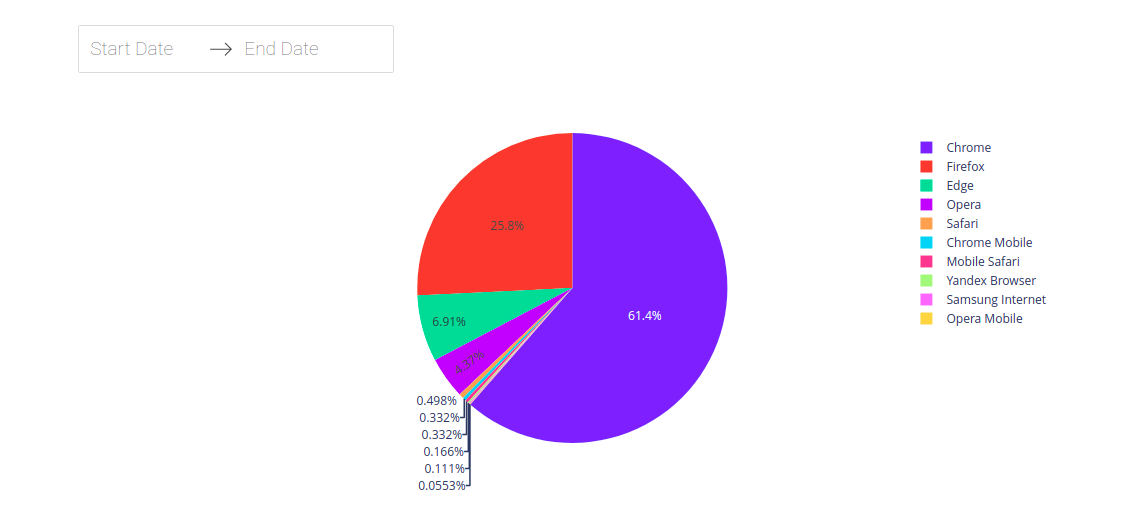
\includegraphics[width=18cm, keepaspectratio]{img/browser.png}
    \caption{Gráfico de navegadores}
    \label{fig:browser}
\end{figure}
Se ha creado una gráfica similar a la anterior para representar los Sistemas Operativos utilizados por los usuarios que acceden a Unibotics, como se puede ver en la Figura \ref{fig:os}. Ambas gráficas tienen filtro por fechas. En ambas gráficas circulares se ha hecho uso del campo \textit{browser} del índice de \texttt{session\_log}, el cual da la información sobre el sistema operativo y el navegador utilizado. Para realizar dichas gráficas circulares se programa el siguiente código:
\begin{verbatim}
def get_temporal_figure__browser(df):
    fig = px.pie(df, values='count', names='browser')
return fig
\end{verbatim}

\begin{figure}[H]
    \centering
    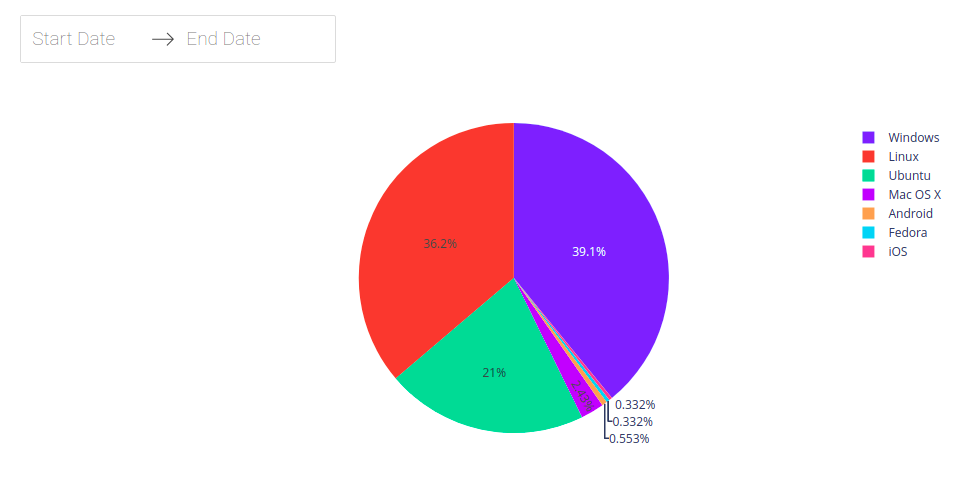
\includegraphics[width=15cm, keepaspectratio]{img/os.png}
    \caption{Gráfico de sistemas operativos}
    \label{fig:os}
\end{figure}
\subsection{Puntuaciones automáticas}
Las siguientes gráficas son las puntuaciones de estilo y eficacia que podrán ser vistas tanto por los usuarios (que pueden acceder a sus puntuaciones) como por los administradores (que pueden acceder a las puntuaciones de todos los usuarios).  Actualmente, las evaluaciones solo están disponibles en cuatro ejercicios. Se representa en una gráfica, en la que cada punto es una evaluación solicitada por el usuario. Las gráficas mostradas en las Figuras \ref{fig:score} y \ref{fig:score_efficacy}  son un ejemplo de las notas de estilo y eficacia de un usuario de la base de datos de prueba en el ejercicio \textit{follow\_line}. Las gráficas de los demás ejercicios son iguales. Para crear estas gráficas se utilizan todos los campos del índice de \texttt{style\_log} y \texttt{efficacy\_log}. El código de ambas gráficas es:
\begin{verbatim}
def score_fig(df):
    fig = px.scatter(df, x="date", y="score")
return fig
\end{verbatim}




\begin{figure}[H]
    \centering
    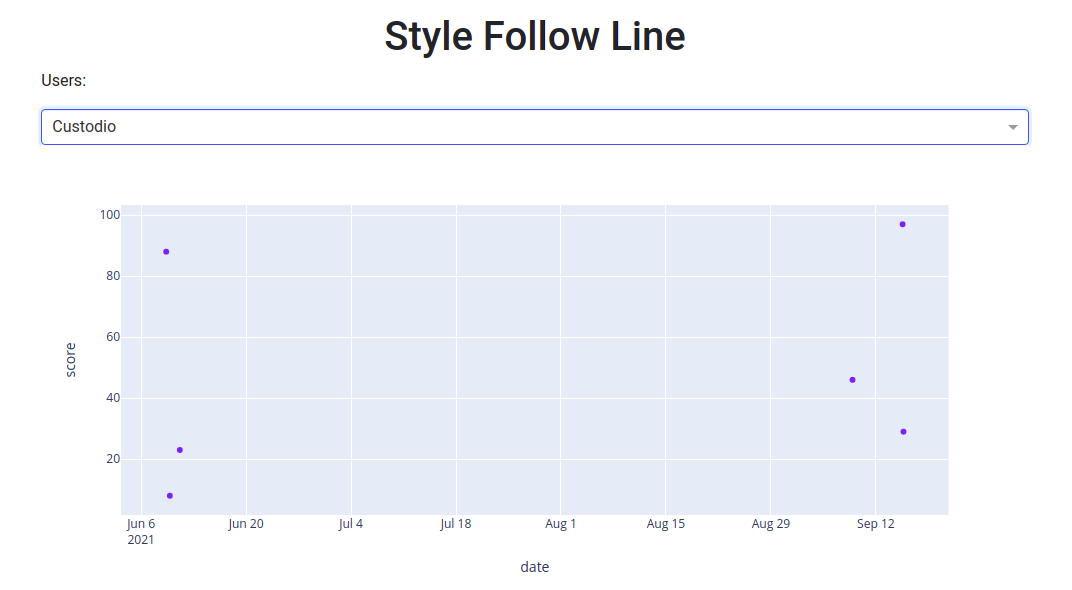
\includegraphics[width=17cm, keepaspectratio]{img/score.png}
    \caption{Gráfica de puntuación de estilo}
    \label{fig:score}
\end{figure}


\begin{figure}[H]
    \centering
    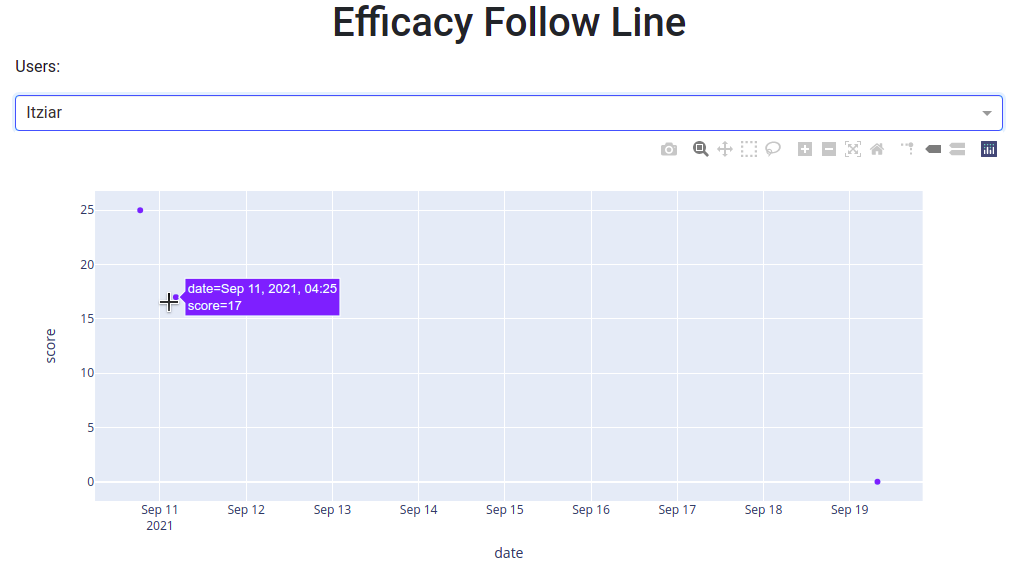
\includegraphics[width=17cm, keepaspectratio]{img/score_efficacy.png}
    \caption{Gráfica de puntuación de eficacia}
    \label{fig:score_efficacy}
\end{figure}




